\chapter{Proposed Work}

\section{Background}
\subsubsection{Intent Detection}
Intent detection can be treated as a semantic utterance classification problem, where the input to the classification model is a sequence of words and the output is the speaker intent class. Given an utterance with a sequence of words $w = (w1, w2, ..., wT)$, the goal of intent detection is to assign an intent class c from a pre-defined finite set of intent classes, such that:
\begin{equation}
\tilde{c} = arg\max_{c} P(c | w)
\end{equation}
Recent neural network based intent classification models involve using neural bag-of-words
(NBoW) or bag-of-n-grams, where words or ngrams are mapped to high dimensional vector
space and then combined component-wise by summation or average before being sent to the
classifier. More structured neural network approaches for utterance classification include using recursive neural network (RecNN) (Guo et al., 2014), recurrent neural network (Ravuri and Stolcke, 2015), and convolutional neural network models (Collobert and Weston, 2008; Kim, 2014). Comparing to basic NBoW methods, these models can better capture the structural patterns in the word sequence.

\subsubsection{Slot Filling}
A major task in spoken language understanding (SLU) is to extract semantic constituents by
searching input text to fill in values for predefined slots in a semantic frame (Mesnil et al.,2015), which is often referred to as slot filling. The slot filling task can also be viewed as assigning an appropriate semantic label to each word in the given input text. In the below example from ATIS (Hemphill et al., 1990) corpus following the popular in/out/begin (IOB) annotation method, Seattle and San Diego are the from and to locations respectively according to the slot labels, and tomorrow is the departure date. Other words in the
example utterance that carry no semantic meaning are assigned “O” label.

\begin{figure}
	\centering
	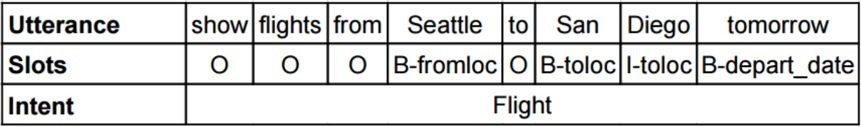
\includegraphics[width=\textwidth]{fig/atis}
	\caption{ATIS corpus sample with intent and slot annotation}
\end{figure}

Given an utterance consisting of a sequence of words $w = (w1, w2, ..., wT)$, the goal of slot filling is to find a sequence of semantic labels $s = (s1, s2, ..., sT)$, one for each word in the utterance, such that:

\begin{equation}
\tilde{s} = arg\max_{s} P(s|w)
\end{equation}

Slot filling is typically treated as a sequence labeling problem. Sequence models including conditional random fields (Raymond and Riccardi, 2007) and RNN models (Yao et al., 2014; Mesnil et al., 2015; Liu and Lane, 2015) are among the most popular methods for sequence labeling tasks.

\subsubsection{RNN Language Model}
A language model assigns a probability to a sequence of words w = (w1, w2, ..., wT ) following
probability distribution. In language modeling, w0 and wT +1 are added to the word sequence representing the beginning-of-sentence token and end-of-sentence token. Using the chain rule, the likelihood of a word sequence can be factorized as:
\begin{equation}
P(w) = \sum_{t=1}^{T} P(w_t|w_0 , ..., w_{t-1})
\end{equation}
RNN-based language models (Mikolov et al.,2011), and the variant (Sundermeyer et al., 2012) using long short-term memory (LSTM) (Hochreiter and Schmidhuber, 1997) have shown superior
performance comparing to traditional n-gram based models. In this work, we use an LSTM cell
as the basic RNN unit for its stronger capability in capturing long-range dependencies in word sequence. 

\subsection{RNN for Intent Detection and Slot Filling}
\begin{figure}
	\centering
	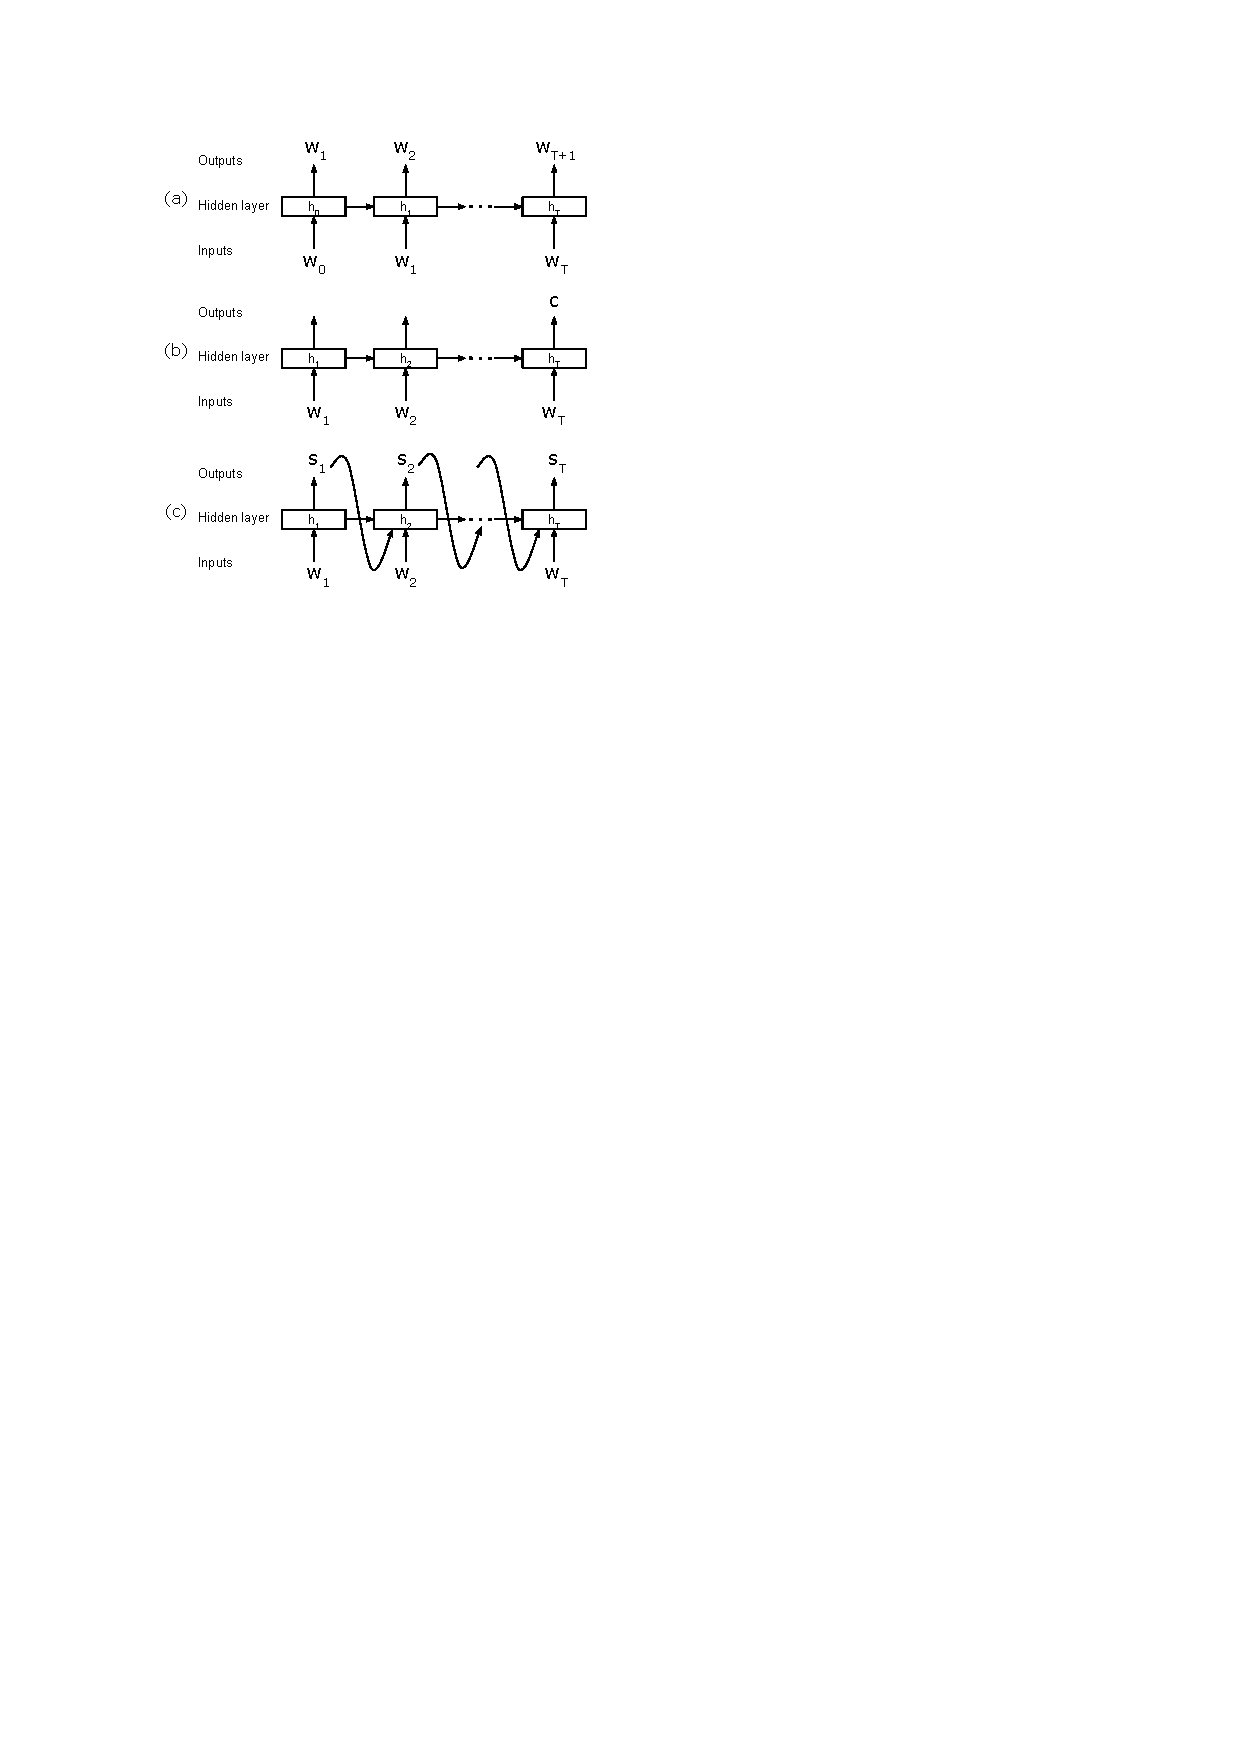
\includegraphics[width=0.6\textwidth]{fig/jslu-rnnmod}
	\caption{(a) RNN language model. (b) RNN intent detection model. The RNN output at last step
		is used to predict the intent class. (c) RNN slot filling model.}
\end{figure}
As illustrated in Figure, RNN intent detection
model uses the last RNN output to predict the utterance
intent class. This last RNN output can be
seen as a representation or embedding of the entire
utterance. Alternatively, the utterance embedding
can be obtained by taking mean of the RNN outputs
over the sequence. This utterance embedding
is then used as input to the multinomial logistic
regression for the intent class prediction.
RNN slot filling model takes word as input and
the corresponding slot label as output at each time
step. The posterior probability for each slot label
is calculated using the softmax function over the
RNN output. Slot label dependencies can be modeled
by feeding the output label from the previous
time step to the current step hidden state (Figure
2(c)). During model training, true label from
previous time step can be fed to current hidden
state. During inference, only the predicted label
can be used. To bridge the gap between training
and inference, scheduled sampling method (Bengio
et al., 2015) can be applied. Instead of only
using previous true label, using sample from previous
predicted label distribution in model training
makes the model more robust by forcing it to
learn to handle its own prediction mistakes (Liu
and Lane, 2015).

\section{Method 1}
In this section we describe the joint SLU-LM model in detail. 
\subsection{Model}
Let $w = (w0, w1, w2, ..., wT+1)$ represent the input word sequence, with w0 and wT +1
being the beginning-of-sentence ($bos$) and end-of-sentence ($eos$) tokens. Let $c =
(c0, c1, c2, ..., cT )$ be the sequence of intent class
outputs at each time step. Similarly, let $s =
(s0, s1, s2, ..., sT )$ be the slot label sequence,
where s0 is a padded slot label that maps to the
beginning-of-sentence token $bos$.
\par
\begin{figure}
	\centering
	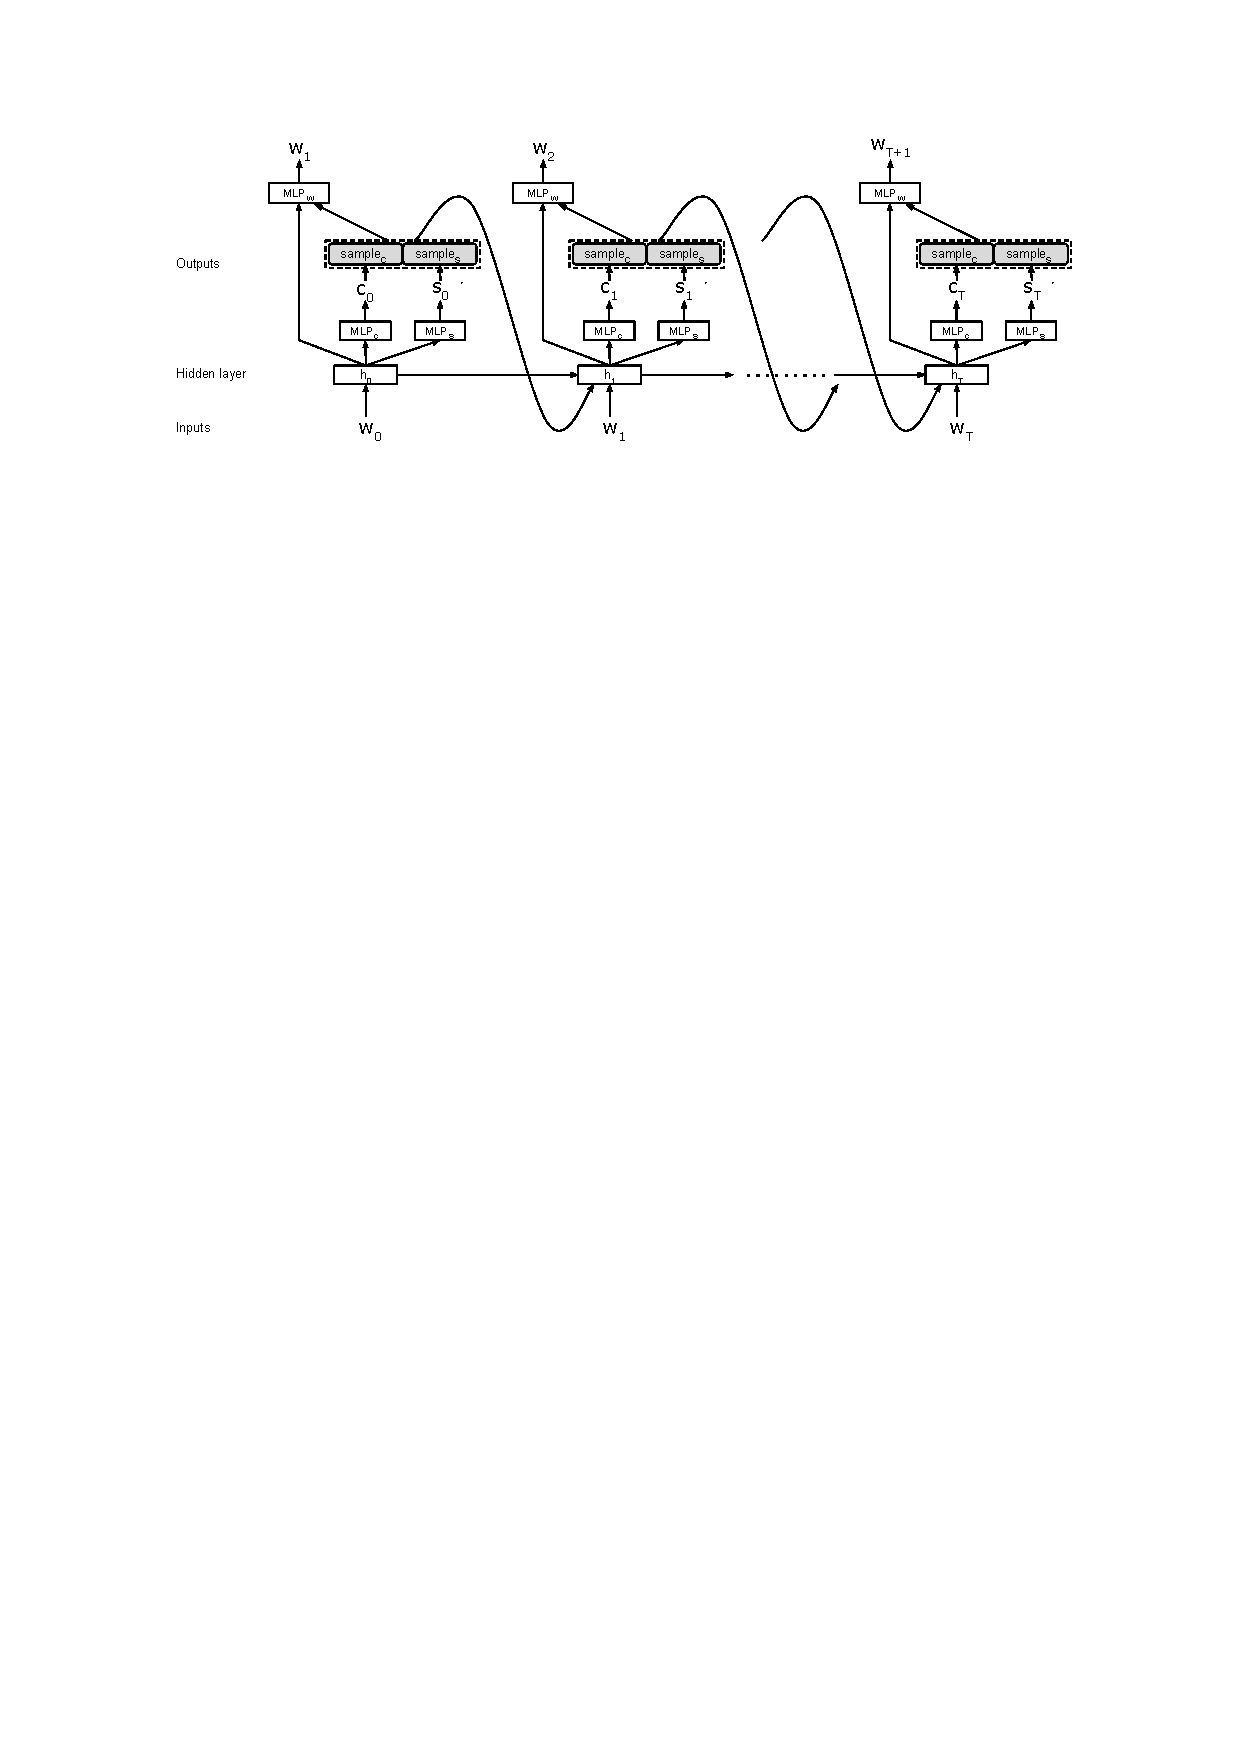
\includegraphics[width=\textwidth]{fig/jslu-mod}
	\caption{Joint online RNN model for intent detection, slot filling, and next word prediction.}
\end{figure}
Referring to the joint SLU-LM model shown in
Figure , for the intent model, instead of predicting
the intent only after seeing the entire utterance
as in the independent training intent model, in the joint model we output intent at each
time step as input word sequence arrives. The intent
generated at the last step is used as the final
utterance intent prediction. The intent output from
each time step is fed back to the RNN state, and
thus the entire intent output history are modeled
and can be used as context to other tasks. It is
not hard to see that during inference, intent classes
that are predicted during the first few time steps
are of lower confidence due to the limited information
available. We describe the techniques that
can be used to ameliorate this effect in section 3.3
below. For the intent model, with both intent and
slot label connections to the RNN state, we have:
\begin{equation}
P(c_T |w) = P(c_T|w \le T,c < T,s < T)
\end{equation}
For the slot filling model, at each step t along the
input word sequence, we want to model the slot
label output st as a conditional distribution over
the previous intents $c<t$, previous slot labels $s<t$,
and the input word sequence up to step t. Using the chain rule, we have:
\begin{equation}
P(s|w) = P(s0|w0) \sum_{t=1}^{T} P(s_t|w≤t, c<t, s<t)
\end{equation}


\subsection{Next Step Prediction}
Following the model architecture in Figure 3, at
time step t, input to the system is the word at index
t of the utterance, and outputs are the intent
class, the slot label, and the next word prediction.
The RNN state ht encodes the information of all
the words, intents, and slot labels seen previously.
The neural network model computes the outputs
through the following sequence of steps:
\begin{eqnarray}
h_t = LSTM(h_{t−1}, [w_t, c_{t−1}, s_{t−1}]) \\
P(c_t|w≤t, c<t, s<t) = IntentDist(h_t) \\
P(s_t|w≤t, c<t, s<t) = SlotLabelDist(h_t)
\end{eqnarray}
where LSTM is the recurrent neural network function
that computes the hidden state $h_t$ at a step
using the previous hidden state $h_{t−1}$, the embeddings
of the previous intent output $c_{t−1}$ and
slot label output $s_{t−1}$, and the embedding of current input word $w_t$. IntentDist, SlotLabelDist are multilayer perceptrons (MLPs) with softmax outputs over intents, slot labels, and words respectively. Each of these three MLPs has
its own set of parameters. The intent and slot label
distributions are generated by the MLPs with input
being the RNN cell output. The next word distribution
is produced by conditioning on current step
RNN cell output together with the embeddings of
the sampled intent and sampled slot label.

\section{Method 2}

\subsection{Model}
The idea of introducing attention to the alignment-based RNN sequence labeling model is motivated by the use of attention mechanism in encoder-decoder models. In bidirectional RNN for sequence labeling,
the hidden state at each time step carries information of the
whole sequence, but information may gradually lose along the
forward and backward propagation. Thus, when making slot label
prediction, instead of only utilizing the aligned hidden state
hi at each step, we would like to see whether the use of context
vector ci gives us any additional supporting information, especially
those require longer term dependencies that is not being
fully captured by the hidden state.
\begin{figure}
	\centering
	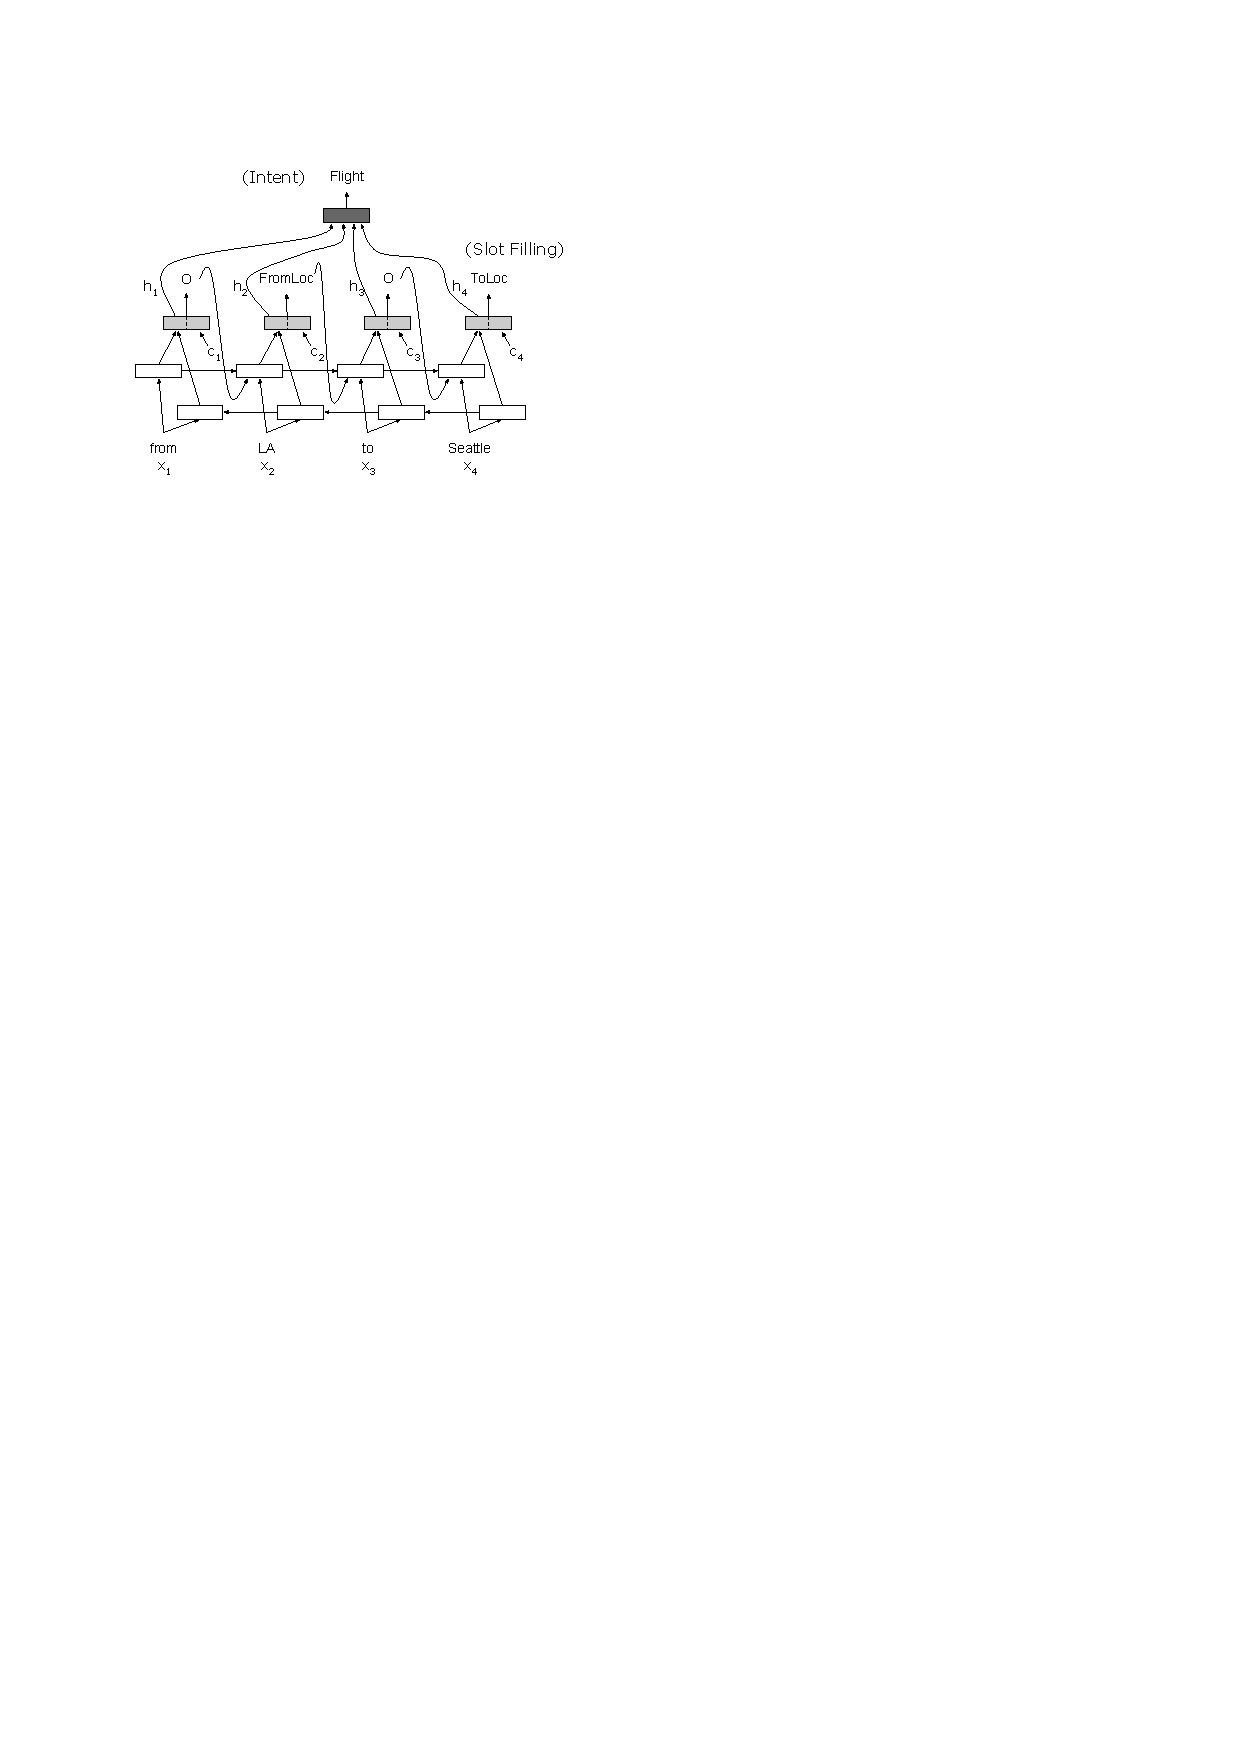
\includegraphics[width=\textwidth]{fig/att-mod}
	\caption[Attention Based RNN Model]{Attention-based RNN model for joint intent detection
		and slot filling. The bidirectional RNN reads the source sequence
		forward and backward. Slot label dependency is modeled
		in the forward RNN. At each time step, the concatenated
		forward and backward hidden states is used to predict the slot
		label. If attention is enabled, the context vector ci provides information
		from parts of the input sequence that is used together
		with the time aligned hidden state hi for slot label prediction.}
\end{figure}
In the proposed model, a bidirectional RNN (BiRNN) reads
the source sequence in both forward and backward directions.
We use LSTM cell for the basic RNN unit. Slot label dependencies
are modeled in the forward RNN. Similar to the encoder
module in the above described encoder-decoder architecture,
the hidden state hi at each step is a concatenation of the forward
state fhi and backward state bhi, hi = [fhi, bhi]. Each
hidden state hi contains information of the whole input word
sequence, with strong focus on the parts surrounding the word
at step i. This hidden state hi is then combined with the context
vector ci to produce the label distribution, where the context
vector ci is calculated as a weighted average of the RNN hidden
states h = (h1, ..., hT ).

For joint modeling of intent detection and slot filling, we
reuse the pre-computed hidden states h of the bidirectional
RNN to produce intent class distribution. If attention is not
used, we apply mean-pooling [17] over time on the hidden
states h followed by logistic regression to perform the intent
classification. If attention is enabled, we instead take the
weighted average of the hidden states h over time.
Comparing to the attention-based encoder-decoder model
that utilizes explicit aligned inputs, the attention-based RNN
model is more computational efficient. During model training,
the encoder-decoder slot filling model reads through the input
sequence twice, while the attention-based RNN model reads
through the input sequence only once.

\subsection{Objective Functions}
\subsubsection{Cross entropy}

Most approaches use a logistic regression classifier with the
softmax activation function in the final layer. The objective
function which is mainly used in this case is based on cross
entropy:
\begin{equation}
L = − \sum_{c} y_c · log(s_\theta(x)c) (4)
\end{equation}
In this equation, c iterates over all classes, $y_c$ is the correct
value for class c and $s$ is the score the network assigned
to class c given the current data point x.

\subsubsection{Ranking}
Instead of using the softmax activation function, we train a matrix $W_{class}$ whose columns contain vector representation of the different classes. Therefore, the score for each class c
can be computed by using the product
\begin{equation}
s_\theta(x)c = h_t^x [W_{class}]c
\end{equation}
We use a ranking loss function to train the RNN. It learns to maximize the distance between the true label y+ and the best competitive label c- given a data point x. The objective function is
\begin{equation}
L = log(1 + exp(\gamma(m+ - s_\theta(x)y+ ))) \\
+ log(1 + exp(\gamma(m- + s_\theta(x)c− )))
\end{equation}
This function was proposed by Dos Santos et al. [23] to train convolution neural networks for
relation classification. The parameter $\gamma$ controls the penalization of the prediction errors and m+ and m- are margins for the correct and incorrect classes. $\gamma$, m+ and m- are hyperparameters which can be tuned on the development set. For the class O, we only calculate the second summand of equation. By doing this, we do not learn a pattern for class O but
nevertheless increase its difference to the best competitive label.

During testing, the model will predict class O if the score
for all the other classes is lower than 0. One of the advantages of this loss function over the softmax function is efficiency. Since only two classes are computed at every training iteration, the network can be trained quite fast even with a large number of classes. Furthermore,
a ranking loss function is suitable for tasks like slot filling because
it does not force the network to learn a pattern for the O
class which in fact may not exist.

\subsection{Training}
The network is trained to find the parameters $\theta$ that minimise the cross-entropy or ranking  of the predicted and true distributions for intent class, slot label, and next word jointly. The objective function also includes an L2 regularization term $R(\theta)$ over the
weights and biases of the three MLPs. This equalizes to finding the parameters $\theta$ that maximize the below objective function:

\begin{equation}
\max_{\theta} \sum_{t=1}^{T} \alpha_c \log P(c^*|w \le t, c<t, s<t; \theta) \\
+ \alpha_s \log P(s^*_t|w \le t, c<t, s<t; \theta) - \lambda R(\theta)
\end{equation}

where c* is the true intent class and and s* is the
true slot label at time step t. $\alpha_c$ and $\alpha_s$ are the
linear interpolation weights for the true intent, slot
label. During model training, $c_t$ can either be the true intent or mixture
of true and predicted intent. During inference,
however, only predicted intent can be used. 
\begin{figure}
	\centering
	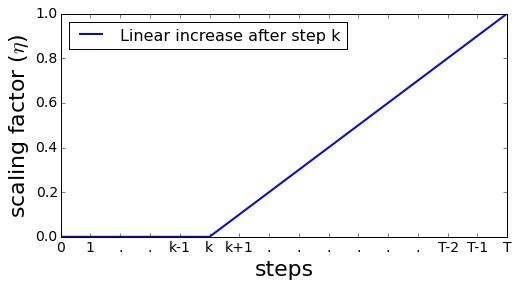
\includegraphics[width=0.5\textwidth]{fig/intent-g}
	\caption{Schedule of increasing intent contribution
		to the context vector along with the growing
		input sequence}
\end{figure}
Confidence of the predicted intent during the first few
time steps is likely to be low due to the limited
information available, and the confidence level is
likely to increase with the newly arriving words.
Conditioning on incorrect intent for next word prediction
is not desirable. To mitigate this effect,
we propose to use a schedule to increase the intent
contribution to the context vector along the
growing input word sequence. Specifically, during
the first k time steps, we disable the intent context
completely by setting the values in the intent
vector to zeros. From step k + 1 till the last step
of the input word sequence, we gradually increase
the intent context by applying a linearly growing
scaling factor $\eta$ from 0 to 1 to the intent vector.

\subsection{Inference}

For online inference, we simply take the greedy path of our conditional model without doing
search. The model emits best intent class and slot label at each time step conditioning on all previous emitted symbols:
\begin{eqnarray}
\tilde{c}_t = arg\max_{c_t} P(c_t|w \le t, \tilde{c}<t, \tilde{s}<t) \\
\tilde{s}_t = arg\max_{s_t} P(s_t|w \le t, \tilde{c}<t, \tilde{c}<t)
\end{eqnarray}
Many applications can benefit from this greedy inference approach comparing to search based inference methods, especially those running on embedded platforms that without GPUs and with limited computational capacity. Alternatively, one can do left-to-right beam search (Sutskever et al., 2014; Chan et al., 2015) by maintaining a set of $\beta$ best partial hypotheses at each step. Efficient beam search method for the joint conditional model is left to explore in our future work.


